% Options for packages loaded elsewhere
% Options for packages loaded elsewhere
\PassOptionsToPackage{unicode}{hyperref}
\PassOptionsToPackage{hyphens}{url}
%
\documentclass[
  12pt,
  letterpaper,
  DIV=11,
  numbers=noendperiod]{scrartcl}
\usepackage{xcolor}
\usepackage[left=1in,right=1in,top=1in,bottom=1in]{geometry}
\usepackage{amsmath,amssymb}
\setcounter{secnumdepth}{5}
\usepackage{iftex}
\ifPDFTeX
  \usepackage[T1]{fontenc}
  \usepackage[utf8]{inputenc}
  \usepackage{textcomp} % provide euro and other symbols
\else % if luatex or xetex
  \usepackage{unicode-math} % this also loads fontspec
  \defaultfontfeatures{Scale=MatchLowercase}
  \defaultfontfeatures[\rmfamily]{Ligatures=TeX,Scale=1}
\fi
\usepackage{lmodern}
\ifPDFTeX\else
  % xetex/luatex font selection
  \setmainfont[ItalicFont=EB Garamond Italic,BoldFont=EB Garamond
SemiBold]{EB Garamond Math}
  \setsansfont[]{EB Garamond SemiBold}
  \setmathfont[]{EB Garamond Math}
\fi
% Use upquote if available, for straight quotes in verbatim environments
\IfFileExists{upquote.sty}{\usepackage{upquote}}{}
\IfFileExists{microtype.sty}{% use microtype if available
  \usepackage[]{microtype}
  \UseMicrotypeSet[protrusion]{basicmath} % disable protrusion for tt fonts
}{}
\usepackage{setspace}
% Make \paragraph and \subparagraph free-standing
\makeatletter
\ifx\paragraph\undefined\else
  \let\oldparagraph\paragraph
  \renewcommand{\paragraph}{
    \@ifstar
      \xxxParagraphStar
      \xxxParagraphNoStar
  }
  \newcommand{\xxxParagraphStar}[1]{\oldparagraph*{#1}\mbox{}}
  \newcommand{\xxxParagraphNoStar}[1]{\oldparagraph{#1}\mbox{}}
\fi
\ifx\subparagraph\undefined\else
  \let\oldsubparagraph\subparagraph
  \renewcommand{\subparagraph}{
    \@ifstar
      \xxxSubParagraphStar
      \xxxSubParagraphNoStar
  }
  \newcommand{\xxxSubParagraphStar}[1]{\oldsubparagraph*{#1}\mbox{}}
  \newcommand{\xxxSubParagraphNoStar}[1]{\oldsubparagraph{#1}\mbox{}}
\fi
\makeatother


\usepackage{longtable,booktabs,array}
\usepackage{calc} % for calculating minipage widths
% Correct order of tables after \paragraph or \subparagraph
\usepackage{etoolbox}
\makeatletter
\patchcmd\longtable{\par}{\if@noskipsec\mbox{}\fi\par}{}{}
\makeatother
% Allow footnotes in longtable head/foot
\IfFileExists{footnotehyper.sty}{\usepackage{footnotehyper}}{\usepackage{footnote}}
\makesavenoteenv{longtable}
\usepackage{graphicx}
\makeatletter
\newsavebox\pandoc@box
\newcommand*\pandocbounded[1]{% scales image to fit in text height/width
  \sbox\pandoc@box{#1}%
  \Gscale@div\@tempa{\textheight}{\dimexpr\ht\pandoc@box+\dp\pandoc@box\relax}%
  \Gscale@div\@tempb{\linewidth}{\wd\pandoc@box}%
  \ifdim\@tempb\p@<\@tempa\p@\let\@tempa\@tempb\fi% select the smaller of both
  \ifdim\@tempa\p@<\p@\scalebox{\@tempa}{\usebox\pandoc@box}%
  \else\usebox{\pandoc@box}%
  \fi%
}
% Set default figure placement to htbp
\def\fps@figure{htbp}
\makeatother


% definitions for citeproc citations
\NewDocumentCommand\citeproctext{}{}
\NewDocumentCommand\citeproc{mm}{%
  \begingroup\def\citeproctext{#2}\cite{#1}\endgroup}
\makeatletter
 % allow citations to break across lines
 \let\@cite@ofmt\@firstofone
 % avoid brackets around text for \cite:
 \def\@biblabel#1{}
 \def\@cite#1#2{{#1\if@tempswa , #2\fi}}
\makeatother
\newlength{\cslhangindent}
\setlength{\cslhangindent}{1.5em}
\newlength{\csllabelwidth}
\setlength{\csllabelwidth}{3em}
\newenvironment{CSLReferences}[2] % #1 hanging-indent, #2 entry-spacing
 {\begin{list}{}{%
  \setlength{\itemindent}{0pt}
  \setlength{\leftmargin}{0pt}
  \setlength{\parsep}{0pt}
  % turn on hanging indent if param 1 is 1
  \ifodd #1
   \setlength{\leftmargin}{\cslhangindent}
   \setlength{\itemindent}{-1\cslhangindent}
  \fi
  % set entry spacing
  \setlength{\itemsep}{#2\baselineskip}}}
 {\end{list}}
\usepackage{calc}
\newcommand{\CSLBlock}[1]{\hfill\break\parbox[t]{\linewidth}{\strut\ignorespaces#1\strut}}
\newcommand{\CSLLeftMargin}[1]{\parbox[t]{\csllabelwidth}{\strut#1\strut}}
\newcommand{\CSLRightInline}[1]{\parbox[t]{\linewidth - \csllabelwidth}{\strut#1\strut}}
\newcommand{\CSLIndent}[1]{\hspace{\cslhangindent}#1}



\setlength{\emergencystretch}{3em} % prevent overfull lines

\providecommand{\tightlist}{%
  \setlength{\itemsep}{0pt}\setlength{\parskip}{0pt}}



 


\setlength\heavyrulewidth{0ex}
\setlength\lightrulewidth{0ex}
\KOMAoption{captions}{tableheading}
\makeatletter
\@ifpackageloaded{caption}{}{\usepackage{caption}}
\AtBeginDocument{%
\ifdefined\contentsname
  \renewcommand*\contentsname{Table of contents}
\else
  \newcommand\contentsname{Table of contents}
\fi
\ifdefined\listfigurename
  \renewcommand*\listfigurename{List of Figures}
\else
  \newcommand\listfigurename{List of Figures}
\fi
\ifdefined\listtablename
  \renewcommand*\listtablename{List of Tables}
\else
  \newcommand\listtablename{List of Tables}
\fi
\ifdefined\figurename
  \renewcommand*\figurename{Figure}
\else
  \newcommand\figurename{Figure}
\fi
\ifdefined\tablename
  \renewcommand*\tablename{Table}
\else
  \newcommand\tablename{Table}
\fi
}
\@ifpackageloaded{float}{}{\usepackage{float}}
\floatstyle{ruled}
\@ifundefined{c@chapter}{\newfloat{codelisting}{h}{lop}}{\newfloat{codelisting}{h}{lop}[chapter]}
\floatname{codelisting}{Listing}
\newcommand*\listoflistings{\listof{codelisting}{List of Listings}}
\makeatother
\makeatletter
\makeatother
\makeatletter
\@ifpackageloaded{caption}{}{\usepackage{caption}}
\@ifpackageloaded{subcaption}{}{\usepackage{subcaption}}
\makeatother
\usepackage{bookmark}
\IfFileExists{xurl.sty}{\usepackage{xurl}}{} % add URL line breaks if available
\urlstyle{same}
\hypersetup{
  pdftitle={When are Philosophy Articles Cited?},
  pdfauthor={Anon},
  hidelinks,
  pdfcreator={LaTeX via pandoc}}


\title{When are Philosophy Articles Cited?}
\author{Anon}
\date{2025-06-16}
\begin{document}
\maketitle
\begin{abstract}
It's natural to believe that philosophy citations are typically to long
ago pieces. We're still talking about philosophers from millenia ago.
More strikingly, we're still talking about papers from half a century
ago not as historical papers, but as part of the contemporary debate.
But a systematic look at the citation data shows that these cases are
outliers. Most citations are to recently published works. Surprisingly,
this is less true in recent years than it used to be. The effect of
electronic publishing and communication has been to make citations, on
average, older. After we adjust for the typical age of philosophy
citations, and this changing trend, it turns out that the 2000s were a
particularly influential time in philosophy publishing. Articles
published in that decade are cited more than earlier or later articles,
once we adjust for the typical times articles are cited, and the
changing patterns of citation. This is arguably related to broad changes
in the interests of philosophers, towards social philosophy, and
epistemology.
\end{abstract}


\setstretch{1.75}
\section{Introduction}\label{sec-introduction}

This paper is about the patterns of citations of philosophy journal
articles in philosophy journals. Obviously philosophy journals cite more
things than philosophy journals, and just as obviously philosophy
journal articles get cited in other places. But looking just at
journal-to-journal citations allows us to get a citation set that is
relatively complete, and hence make some systematic generalisations
about the way articles are cited over time. It turns out some of these
generalisations are surprising.

Before looking at the data, here are two things I believed about
philosophy citations. First, philosophers tend to cite very old papers.
We still regularly teach a number of papers over half a century old in
introductory classes; e.g., H. G. Frankfurt
(\citeproc{ref-WOSA1969Y444700002}{1969}), Thomson
(\citeproc{ref-WOSA1971Y116900003}{1971}), Singer
(\citeproc{ref-WOSA1972Z066400001}{1972}), and Lewis
(\citeproc{ref-10.2307_2025310}{1973a}). These aren't taught as history
papers, but as early entries into the contemporary philosophical debate.
While most papers aren't cited as much as these papers are, I thought
the pattern that old papers keep being cited extended to their less
famous counterparts. Second, the technological changes of the last
quarter century meant that this practice was being slowly reversed. A
series of technological innovations made it easier to cite newer and
newer works. These innovations included the spread of email, the rise of
preprint archives (e.g., arXiv, SSRN, PhilPapers), and eventually
official preprints in things like EarlyView. So, I thought, citations
should be getting younger, because the delay between publishing and
getting widely known was removed.

Both of these thoughts were wrong.

On the first point, the generalisation I made from those famous papers
was just wrong. Normal papers differ from famous papers not just in how
often they are cited, but in the shape of their citations. The main
evidence I'll use for this is something I'll call the \emph{citation
ratio}. The citation ratio of year \emph{o} in year \emph{n} is the mean
number of citations, in year \emph{n}, of articles published in year
\emph{o}, divided by the mean number of citations, in year \emph{n}, of
articles published in years \emph{n}-10 to \emph{n}-3. (I'll say much
more about why I'm using this measure in what follows.)
Figure~\ref{fig-master-citation-ratio} shows the average citation ratio
for different \emph{ages}, of citations, i.e., the number of years
between \emph{o} and \emph{n}.\footnote{The graph also includes some
  `jitter' to make the different points more easily visible. I've put
  each decade of original publication in a different colour; I'll break
  those out in Figure~\ref{fig-decades-cite-ratio}. The graph starts in
  1975 because the data is much noisier before then, for reasons we'll
  get to below.}

\begin{figure}

\centering{

\pandocbounded{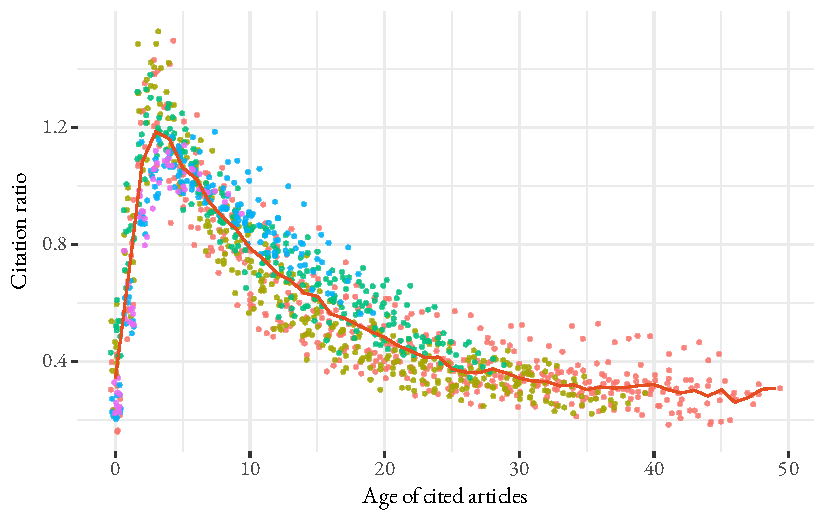
\includegraphics[keepaspectratio]{apc-2025-june-draft_files/figure-pdf/fig-master-citation-ratio-1.pdf}}

}

\caption{\label{fig-master-citation-ratio}Age effects from 1975 onwards
on a single graph, with the overall average shown.}

\end{figure}%

Each dot on that graph is a citation ratio for a particular pair of
years; the line shows the average citation ratio for all pairs with the
same age. The shape is unmistakable; articles get cited much much more
when they are relatively young than when they are older.

The `evidence' I gave for the opposite view in the introductory
paragraph wasn't entirely wrong. If we redo
Figure~\ref{fig-master-citation-ratio} just looking at articles which
have 15 or more citations in philosophy journals. (This turns out to be
a fairly small percentage of the sample.)

\begin{figure}

\centering{

\pandocbounded{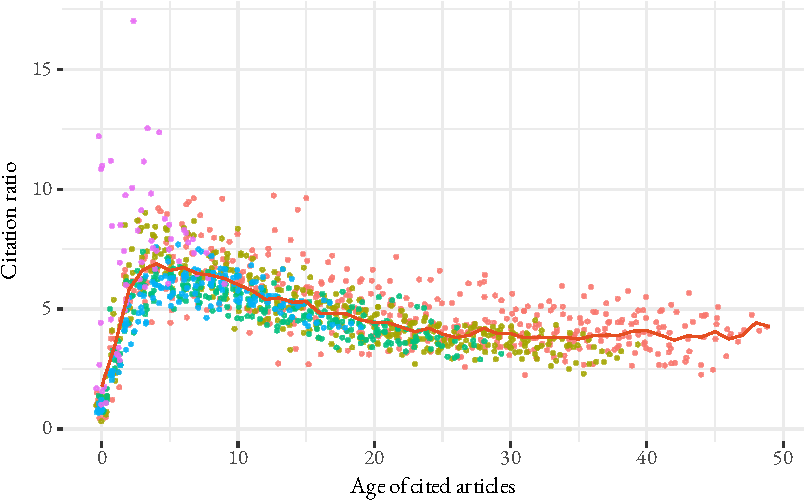
\includegraphics[keepaspectratio]{apc-2025-june-draft_files/figure-pdf/fig-ageeffecteverything-high-1.pdf}}

}

\caption{\label{fig-ageeffecteverything-high}A version of
Figure~\ref{fig-master-citation-ratio} just looking at highly cited
articles}

\end{figure}%

The numbers on the y-axis in Figure~\ref{fig-ageeffecteverything-high}
are higher than in Figure~\ref{fig-master-citation-ratio}. That's not
surprising; it just means highly cited articles get cited more
frequently. What is striking is the different shape of the graphs.
Typical philosophy articles, if they get cited at all, get cited soon
after publication and they fade into obscurity. Highly cited articles
keep getting cited decades after their publication.

These results aren't a priori obvious; things could have turned out
otherwise. It could have been that there were a trove of articles which
were ignored after publication and then accrued five to ten citations a
couple of decades later. There are some articles that were very
frequently cited soon after publication but which are now largely
ignored. (This happens most frequently in philosophy of science and in
philosophy of mind, I think for different reasons in the two cases.) But
these cases are outliers. Most of the articles that were influential
soon after publication stay that way.

For the second point, we can simply break up
Figure~\ref{fig-master-citation-ratio} by ten year chunks. In
Figure~\ref{fig-decades-cite-ratio} I've taken the points by from
Figure~\ref{fig-master-citation-ratio}, and grouped them into `decades'.
Because I'm working here with 1975-2024 data, the decades are 1975-1984,
1985-1994 etc. To make it easier to compare decades, I've removed the
last one, where there isn't enough data, and removed all points with an
age over 20.

\begin{figure}

\begin{minipage}{0.50\linewidth}

\centering{

\pandocbounded{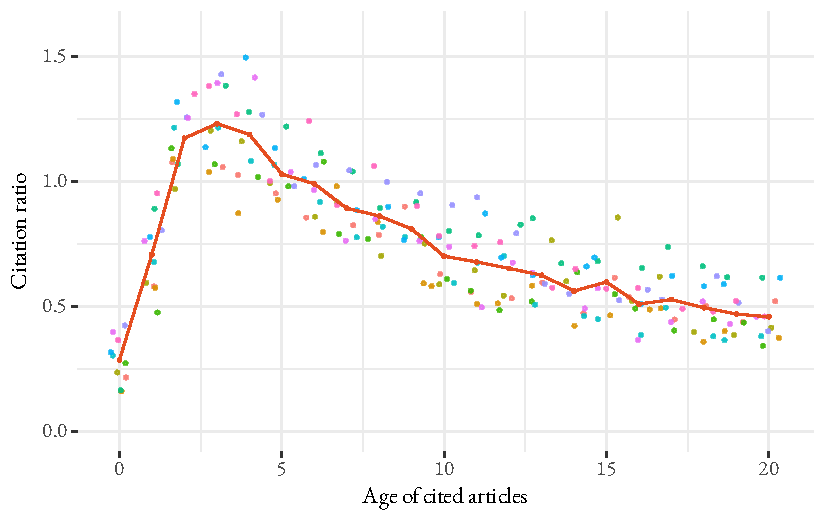
\includegraphics[keepaspectratio]{apc-2025-june-draft_files/figure-pdf/fig-decades-cite-ratio-1.pdf}}

}

\subcaption{\label{fig-decades-cite-ratio-1}1975-1984}

\end{minipage}%
%
\begin{minipage}{0.50\linewidth}

\centering{

\pandocbounded{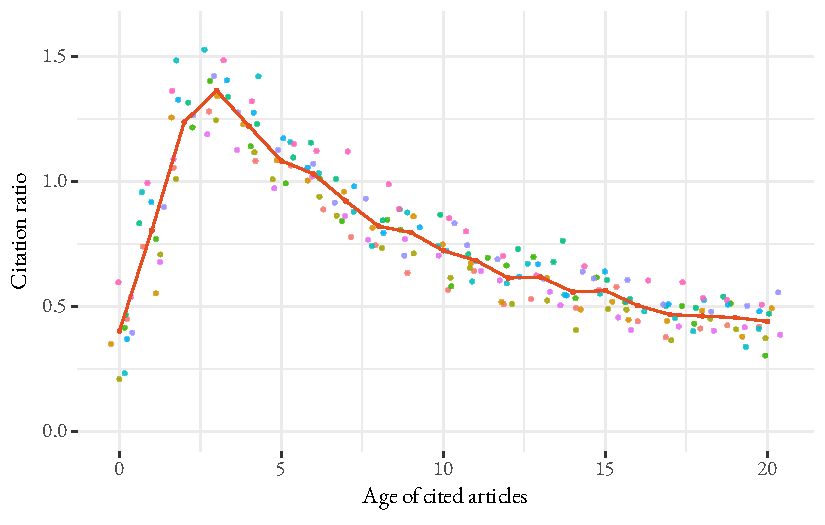
\includegraphics[keepaspectratio]{apc-2025-june-draft_files/figure-pdf/fig-decades-cite-ratio-2.pdf}}

}

\subcaption{\label{fig-decades-cite-ratio-2}1985-1994}

\end{minipage}%
\newline
\begin{minipage}{0.50\linewidth}

\centering{

\pandocbounded{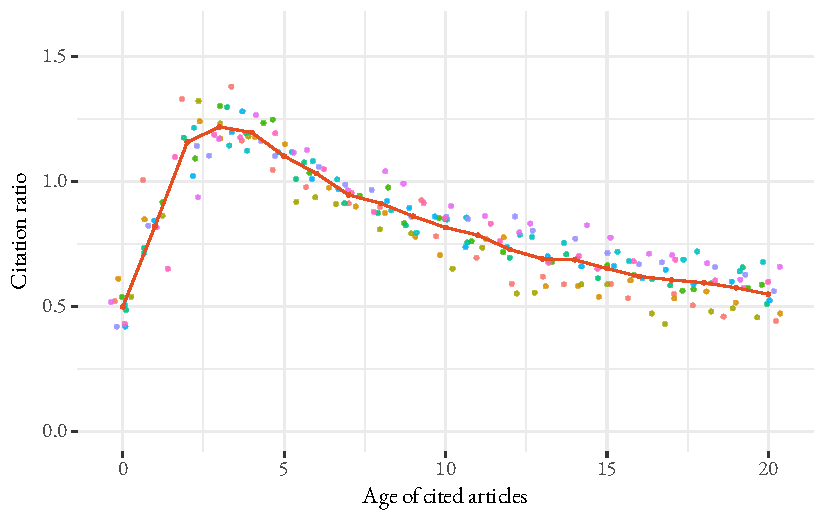
\includegraphics[keepaspectratio]{apc-2025-june-draft_files/figure-pdf/fig-decades-cite-ratio-3.pdf}}

}

\subcaption{\label{fig-decades-cite-ratio-3}1995-2004}

\end{minipage}%
%
\begin{minipage}{0.50\linewidth}

\centering{

\pandocbounded{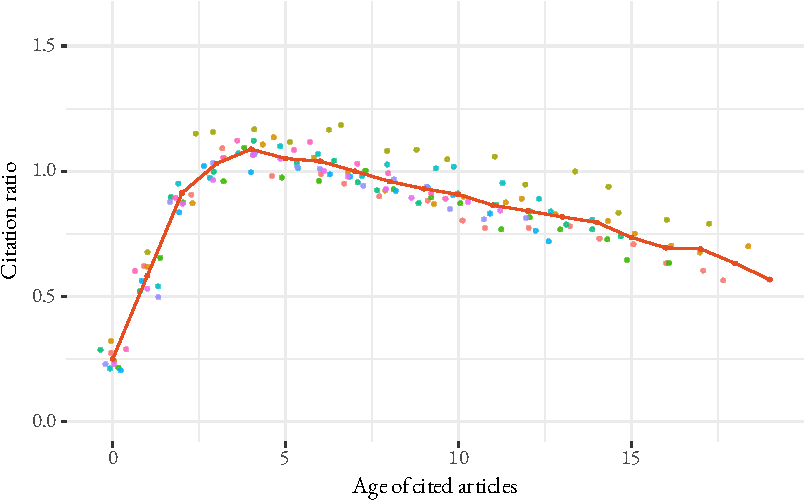
\includegraphics[keepaspectratio]{apc-2025-june-draft_files/figure-pdf/fig-decades-cite-ratio-4.pdf}}

}

\subcaption{\label{fig-decades-cite-ratio-4}2005-2014}

\end{minipage}%

\caption{\label{fig-decades-cite-ratio}Citation ratio for different
decades}

\end{figure}%

There are three general trends across these graphs, especially after the
second graph.

\begin{enumerate}
\def\labelenumi{\arabic{enumi}.}
\tightlist
\item
  The peaks are getting later. In the first two graphs, the line is
  clearly heading down by age 5; in the last one it is barely off the
  peak.
\item
  The peaks are getting lower. In the last graph we barely see it cross
  1.
\item
  The declines are much, much flatter. If you look around age 15 in the
  four graphs, you see the values rise steadily over time.
\end{enumerate}

What all this means is that citations are getting older. While it's
still true that articles from a year are (collectively) cited a more
often from ages 2-5 than from ages 12-15, the difference between those
two rates has fallen remarkably. The effect of technology on citations
has been the complete opposite of what I expected.

The rest of this paper has two aims.

First, I'm going to set out the methodology behind these graphs, go over
the choices I made in building them, and argue that these were at least
defensible choices. The intended conclusion is that these graphs really
show what I say they do, that traditionally citations were mostly to
very recent articles, but they are now more frequently to older
articles.

Second, I'm going to look citations from various years, after adjusting
for these typical citation rates, and see which years have been more
influential in the later literature. I suspect readers will not be
surprised that the early 1970s stand out as being particularly
influential. What might be more surprising is that the next most
influential period, in terms of how often articles from then are cited
compared to the overall trends, is the 2000s. There are a few possible
reasons for this, but I suspect the main one is the rising importance at
that time of epistemology. (This is something Eugenio Petrovich
(\citeproc{ref-Petrovich2024}{2024}) also found using a somewhat
different data set.) More generally, looking at citations from different
periods, and especially looking at which articles make up those
citations, is a useful guide to the history of those periods. Most work
on the history of analytic philosophy doesn't get beyond the early
1970s; this is an early attempt to quantify what happens in the years
after the changes brought about by Kripke, Lewis, Rawls and others in
those years.

\section{Age of Citations}\label{sec-age}

\subsection{Methodology}\label{sec-methodology}

The data for this study comes from Web of Science (hereafter, WoS). In
this section I'll go over which data I chose to use, and how I patched
it together.

The bulk of the data comes from the XML files that WoS makes available
to subscribing institutions. Until recently, that included my own, so
that's where most of the data through 2021 comes from. That subscription
has not been renewed, so the data since 2021 comes from the WoS
API.\footnote{This is also via a susbcription through my institution;
  the XML is more expensive.}

The XML file is rather large. After de-compression it's over a terabyte.
To make it manageable, I filtered down to \emph{articles} (as opposed to
discussion notes, book reviews, editorial matters, and so on), and whose
category was either Philosophy or History \& Philosophy of Science. I
then selected by hand the hundred journals with the most inbound
citations (among articles in these categories) which were (a) primarily
English language, (b) not primarily history of science and (c) broadly
`analytic' rather than `continental'. These were somewhat subjective
choices, but the result was a reasonable collection of the journals
which are most important for telling the story of a certain kind of
philosophy over the last several decades.

The list of journals being used, as well as some basic statistical
information about them, is in \textbf{?@sec-appendix}.

In that appendix I've also included some more details about precise what
was and wasn't included. The most important thing to know is that the
study only considers years of a journal that are indexed by WoS. This
typically starts several years after the journal is founded. For
example, it only starts indexing \emph{Mind \& Language} in 1994,
although the journal is founded eight years earlier.

\begin{longtable}[]{@{}
  >{\raggedright\arraybackslash}p{(\linewidth - 6\tabcolsep) * \real{0.5747}}
  >{\raggedleft\arraybackslash}p{(\linewidth - 6\tabcolsep) * \real{0.1034}}
  >{\raggedleft\arraybackslash}p{(\linewidth - 6\tabcolsep) * \real{0.1264}}
  >{\raggedleft\arraybackslash}p{(\linewidth - 6\tabcolsep) * \real{0.1954}}@{}}

\caption{\label{tbl-list-of-journals}The journals included in this
study.}

\tabularnewline

\toprule\noalign{}
\begin{minipage}[b]{\linewidth}\raggedright
Journal
\end{minipage} & \begin{minipage}[b]{\linewidth}\raggedleft
Articles
\end{minipage} & \begin{minipage}[b]{\linewidth}\raggedleft
First Year
\end{minipage} & \begin{minipage}[b]{\linewidth}\raggedleft
Most Recent Year
\end{minipage} \\
\midrule\noalign{}
\endhead
\bottomrule\noalign{}
\endlastfoot
American Philosophical Quarterly & 1835 & 1964 & 2024 \\
Analysis & 2719 & 1975 & 2024 \\
Analytic Philosophy & 190 & 2016 & 2024 \\
Archiv für Geschichte der Philosophie & 672 & 1975 & 2024 \\
Australasian Journal of Philosophy & 1736 & 1975 & 2024 \\
Biology and Philosophy & 1225 & 1988 & 2024 \\
British Journal for the History of Philosophy & 834 & 2007 & 2024 \\
British Journal for the Philosophy of Science & 1620 & 1956 & 2024 \\
British Journal of Aesthetics & 1436 & 1975 & 2024 \\
Bulletin of Symbolic Logic & 443 & 1997 & 2024 \\
Canadian Journal of Philosophy & 1552 & 1975 & 2023 \\
Croatian Journal of Philosophy & 376 & 2007 & 2024 \\
Dialogue & 1555 & 1975 & 2024 \\
Economics and Philosophy & 568 & 1986 & 2024 \\
Episteme & 586 & 2005 & 2024 \\
Ergo & 386 & 2016 & 2024 \\
Erkenntnis & 1780 & 2000 & 2024 \\
Ethical Theory and Moral Practice & 902 & 2008 & 2024 \\
Ethics & 1673 & 1955 & 2024 \\
Ethics and Information Technology & 567 & 2001 & 2024 \\
European Journal for Philosophy of Science & 562 & 2011 & 2024 \\
European Journal of Philosophy & 994 & 1998 & 2024 \\
Heythrop Journal & 1559 & 1975 & 2024 \\
History and Philosophy of Logic & 522 & 1992 & 2024 \\
Hypatia & 683 & 2009 & 2024 \\
Inquiry & 1646 & 1966 & 2024 \\
International Journal for Philosophy of Religion & 1149 & 1975 & 2024 \\
International Philosophical Quarterly & 1588 & 1961 & 2023 \\
Journal of Aesthetics and Art Criticism & 1539 & 1975 & 2024 \\
Journal of Applied Philosophy & 666 & 2006 & 2024 \\
Journal of Chinese Philosophy & 1278 & 1973 & 2024 \\
Journal of Consciousness Studies & 1525 & 2000 & 2024 \\
Journal of Indian Philosophy & 1107 & 1975 & 2024 \\
Journal of Medical Ethics & 4340 & 1975 & 2024 \\
Journal of Moral Philosophy & 392 & 2005 & 2024 \\
Journal of Philosophical Logic & 1497 & 1972 & 2024 \\
Journal of Philosophical Research & 463 & 2005 & 2024 \\
Journal of Philosophy & 2761 & 1956 & 2024 \\
Journal of Political Philosophy & 609 & 1998 & 2023 \\
Journal of Social Philosophy & 508 & 2008 & 2024 \\
Journal of Symbolic Logic & 4363 & 1966 & 2024 \\
Journal of Value Inquiry & 1369 & 1980 & 2024 \\
Journal of the American Philosophical Association & 340 & 2015 & 2024 \\
Journal of the History of Ideas & 2212 & 1956 & 2024 \\
Journal of the History of Philosophy & 1138 & 1975 & 2024 \\
Journal of the Philosophy of History & 284 & 2010 & 2024 \\
Kant-Studien & 1134 & 1975 & 2024 \\
Kantian Review & 337 & 2010 & 2024 \\
Kennedy Institute of Ethics Journal & 574 & 1995 & 2024 \\
Law and Philosophy & 852 & 1982 & 2024 \\
Linguistics and Philosophy & 878 & 1979 & 2024 \\
Logique et Analyse & 340 & 2007 & 2021 \\
Metaphilosophy & 1562 & 1975 & 2024 \\
Mind & 1980 & 1956 & 2024 \\
Mind \& Language & 893 & 1994 & 2024 \\
Minds and Machines & 756 & 1992 & 2024 \\
Monist & 1975 & 1963 & 2024 \\
Notre Dame Journal of Formal Logic & 486 & 2009 & 2024 \\
Noûs & 1480 & 1975 & 2024 \\
Pacific Philosophical Quarterly & 1231 & 1980 & 2024 \\
Philosophers' Imprint & 402 & 2010 & 2024 \\
Philosophia & 2249 & 1975 & 2024 \\
Philosophia Mathematica & 243 & 2008 & 2024 \\
Philosophical Explorations & 390 & 2008 & 2024 \\
Philosophical Forum & 851 & 1971 & 2024 \\
Philosophical Investigations & 708 & 1983 & 2024 \\
Philosophical Papers & 234 & 2009 & 2023 \\
Philosophical Perspectives & 305 & 2007 & 2023 \\
Philosophical Psychology & 1312 & 1991 & 2024 \\
Philosophical Quarterly & 1450 & 1975 & 2024 \\
Philosophical Review & 1033 & 1956 & 2024 \\
Philosophical Studies & 5485 & 1956 & 2024 \\
Philosophy & 1811 & 1956 & 2024 \\
Philosophy \& Public Affairs & 733 & 1971 & 2024 \\
Philosophy Compass & 651 & 2015 & 2024 \\
Philosophy East and West & 1604 & 1966 & 2024 \\
Philosophy and Phenomenological Research & 3273 & 1956 & 2024 \\
Philosophy and Rhetoric & 927 & 1975 & 2024 \\
Philosophy of Science & 3259 & 1956 & 2024 \\
Philosophy of the Social Sciences & 997 & 1975 & 2024 \\
Phronesis & 783 & 1975 & 2024 \\
Politics, Philosophy and Economics & 325 & 2008 & 2024 \\
Ratio & 1090 & 1974 & 2024 \\
Res Philosophica & 360 & 2013 & 2024 \\
Review of Metaphysics & 1616 & 1956 & 2024 \\
Review of Symbolic Logic & 578 & 2008 & 2024 \\
Russell & 345 & 1981 & 2024 \\
Social Epistemology & 489 & 2011 & 2024 \\
Social Philosophy and Policy & 973 & 1983 & 2024 \\
South African Journal of Philosophy & 793 & 1987 & 2024 \\
Southern Journal of Philosophy & 1984 & 1976 & 2024 \\
Studia Logica & 734 & 2010 & 2024 \\
Studies in History and Philosophy of Science & 1832 & 1974 & 2024 \\
Synthese & 7770 & 1966 & 2024 \\
Theoria & 459 & 2007 & 2024 \\
Theory and Decision & 1936 & 1970 & 2024 \\
Thought & 219 & 2016 & 2022 \\
Topoi & 1327 & 1982 & 2024 \\
Transactions of the Charles S. Peirce Society & 1176 & 1975 & 2024 \\
Utilitas & 391 & 2009 & 2024 \\

\end{longtable}

The column `First Year' is \emph{not} the first year the journal
published; it is the first year that Web of Science indexed the journal.
This often makes a difference; because \emph{Analysis} isn't indexed
before 1975, we don't get ``Is Knowledge Justified True Belief?''
(\citeproc{ref-Gettier1963}{Gettier 1963}), or much of the initial
literature it generated. Still, we do have a lot of information to work
with, as long as we're careful about the limitations. Similarly, the
column `Last Year' is not the last year the journal was published;
thankfully most of these journals are still in operation. It's not even
the last year that Web of Science has records for. For most of the
journals, there were records for 2022, and even occasional records for
2023. But I stopped the study in 2021 because it was the last year we
had something that felt close enough to a full year's data.

The database is supposed to tell you, for each indexed article, which
things it cites. The reliability of this is mixed, especially with
citations that are in footnotes rather than in a bibliography. And the
data needs a huge amount of cleaning. Eugenio Petrovich
(\citeproc{ref-Petrovich2024}{2024}) did a similar study to this one
focussing on five high profile journals, and his first step was a rather
extensive bit of data cleaning.\footnote{See section 4.2.4 of his book
  for more details on the challenges he faced.}

That said, for one important class of citations the data seems fairly
reliable (at least as far as I could check), and not in need of much
cleaning. When the citation is to another article that Web of Science
indexes, the database includes the internal reference number of the
cited article. By simply filtering for references that have an internal
reference of this kind, we can quickly get a fairly accurate record of
when the articles in Table~\ref{tbl-list-of-journals} cite other
articles on the table.

The upside of this approach, as opposed to the more thorough approach
that Petrovich used, is that it makes it practical to study a hundred
journals over sixty years. The downside is that it means we don't see
citations to anything other than journal articles, and articles in these
journals in particular. Obviously a full study of the citations in
philosophy journals would want to pay some attention to citations of
\emph{Philosophical Investigations}, \emph{A Theory of Justice},
\emph{On the Plurality of Worlds}, and many many other books. This is
not that `full study'. Instead it's an attempt to analyse an important
part of the citation data; a part that happens to be much easier to
access.

So for the most part the method used here is that I downloaded hundreds
of XML files from Web of Science and ran some filters on them. This took
a few hours -- even modern computers struggle to analyse a terabyte's
worth of information quickly -- but it wasn't that sophisticated. There
were only two other things I had to do to fix the data.

The way Web of Science handles the `supplements' to \emph{Noûs}, i.e.,
\emph{Philosophical Perspectives} and \emph{Philosophical Issues}, was a
little uneven. Some years these are recorded as being their own thing,
i.e., with a source name of \emph{Philosophical Perspectives} or
\emph{Philosophical Issues}; and some years they are recorded as special
issues of \emph{Noûs}. When they were listed as special issues, the
citations were extremely unreliable. Some high profile articles are
recorded as having no citations until several years after publication.
The bibliographic information for the articles themselves was also
spotty. So I've manually removed all records that were listed as special
or supplementary issues of \emph{Noûs} (and similarly removed the
citations to those article that did get tracked).

The other big problem is that for several journals, 1974 is missing from
the index. In a couple of cases, 1973 is also missing. And in one very
important case, 1971 and 1972 are missing as well. That `important case'
is \emph{The Journal of Philosophy}. Between 1971 and 1974 it published
groundbreaking articles by Harry H. Frankfurt
(\citeproc{ref-Frankfurt1971}{1971}), George Boolos
(\citeproc{ref-Boolos1971}{1971}), Paul Benacerraf
(\citeproc{ref-Benacerraf1973}{1973}), Jaegwon Kim
(\citeproc{ref-Kim1973}{1973}), Michael Friedman
(\citeproc{ref-Friedman1974}{1974}), Isaac Levi
(\citeproc{ref-Levi1974}{1974}), and David Lewis
(\citeproc{ref-Lewis1971cen}{1971}, \citeproc{ref-Lewis1973ben}{1973b}).
This seemed like a break in the data that needed fixing if I was going
to tell the story correctly. So I used JSTOR to find a full list of
articles (as opposed to notes or book reviews) in \emph{Journal of
Philosophy} in those years, and then looked through the citations in
articles in Table~\ref{tbl-list-of-journals} to see which citations were
to one of those articles. This did mean I was using a different
classification of publications into articles and non-articles, and there
are some odd choices.\footnote{Notably, the JSTOR list seemed to exclude
  the symposium centered around Kenneth Arrow's ``Some
  Ordinalist-Utilitarian Notes on Rawls's Theory of Justice''; I'm not
  sure why that was.} And it meant I had to do a fair bit of data
cleaning just to track down references to those four years.\footnote{A
  non-trivial chunk of the cleaning was sorting through the many and
  varied ways that philosophers have spelled Brian O'Shaughnessy's name
  over the years.} While I've strived to make the data as consistent as
possible with the other years, it's possible that I haven't succeeded,
and some discontinuities around the early 1970s are due to this
discontinuity in how the data was acquired.

\section{Statistics}\label{sec-statistics}

The paper uses the journals shown in
(\citeproc{ref-apptbl-statistics}{\textbf{apptbl-statistics?}}).

\begin{longtable}[]{@{}
  >{\raggedright\arraybackslash}p{(\linewidth - 10\tabcolsep) * \real{0.4274}}
  >{\raggedleft\arraybackslash}p{(\linewidth - 10\tabcolsep) * \real{0.0940}}
  >{\raggedleft\arraybackslash}p{(\linewidth - 10\tabcolsep) * \real{0.0855}}
  >{\raggedleft\arraybackslash}p{(\linewidth - 10\tabcolsep) * \real{0.0769}}
  >{\raggedleft\arraybackslash}p{(\linewidth - 10\tabcolsep) * \real{0.1624}}
  >{\raggedleft\arraybackslash}p{(\linewidth - 10\tabcolsep) * \real{0.1538}}@{}}
\caption{Journals used in this paper}\tabularnewline
\toprule\noalign{}
\begin{minipage}[b]{\linewidth}\raggedright
Journal
\end{minipage} & \begin{minipage}[b]{\linewidth}\raggedleft
First Year
\end{minipage} & \begin{minipage}[b]{\linewidth}\raggedleft
Last Year
\end{minipage} & \begin{minipage}[b]{\linewidth}\raggedleft
Articles
\end{minipage} & \begin{minipage}[b]{\linewidth}\raggedleft
Outbound Citations
\end{minipage} & \begin{minipage}[b]{\linewidth}\raggedleft
Inbound Citations
\end{minipage} \\
\midrule\noalign{}
\endfirsthead
\toprule\noalign{}
\begin{minipage}[b]{\linewidth}\raggedright
Journal
\end{minipage} & \begin{minipage}[b]{\linewidth}\raggedleft
First Year
\end{minipage} & \begin{minipage}[b]{\linewidth}\raggedleft
Last Year
\end{minipage} & \begin{minipage}[b]{\linewidth}\raggedleft
Articles
\end{minipage} & \begin{minipage}[b]{\linewidth}\raggedleft
Outbound Citations
\end{minipage} & \begin{minipage}[b]{\linewidth}\raggedleft
Inbound Citations
\end{minipage} \\
\midrule\noalign{}
\endhead
\bottomrule\noalign{}
\endlastfoot
American Philosophical Quarterly & 1964 & 2024 & 1835 & 7759 & 10295 \\
Analysis & 1975 & 2024 & 2719 & 7494 & 14833 \\
Analytic Philosophy & 2016 & 2024 & 190 & 2218 & 501 \\
Archiv für Geschichte der Philosophie & 1975 & 2024 & 672 & 1598 &
1019 \\
Australasian Journal of Philosophy & 1975 & 2024 & 1736 & 10463 &
13439 \\
Biology and Philosophy & 1988 & 2024 & 1225 & 6179 & 4825 \\
British Journal for the History of Philosophy & 2007 & 2024 & 834 & 2466
& 1113 \\
British Journal for the Philosophy of Science & 1956 & 2024 & 1620 &
9330 & 13032 \\
British Journal of Aesthetics & 1975 & 2024 & 1436 & 3556 & 3614 \\
Bulletin of Symbolic Logic & 1997 & 2024 & 443 & 1326 & 1139 \\
Canadian Journal of Philosophy & 1975 & 2023 & 1552 & 7772 & 5732 \\
Croatian Journal of Philosophy & 2007 & 2024 & 376 & 1901 & 299 \\
Dialogue & 1975 & 2024 & 1555 & 3697 & 1105 \\
Economics and Philosophy & 1986 & 2024 & 568 & 2607 & 2386 \\
Episteme & 2005 & 2024 & 586 & 5196 & 3127 \\
Ergo & 2016 & 2024 & 386 & 5090 & 867 \\
Erkenntnis & 2000 & 2024 & 1780 & 17201 & 7630 \\
Ethical Theory and Moral Practice & 2008 & 2024 & 902 & 5874 & 2153 \\
Ethics & 1955 & 2024 & 1673 & 5762 & 15689 \\
Ethics and Information Technology & 2001 & 2024 & 567 & 1953 & 1032 \\
European Journal for Philosophy of Science & 2011 & 2024 & 562 & 5952 &
1473 \\
European Journal of Philosophy & 1998 & 2024 & 994 & 5839 & 3023 \\
Heythrop Journal & 1975 & 2024 & 1559 & 875 & 355 \\
History and Philosophy of Logic & 1992 & 2024 & 522 & 1447 & 930 \\
Hypatia & 2009 & 2024 & 683 & 1556 & 1711 \\
Inquiry & 1966 & 2024 & 1646 & 7186 & 4545 \\
International Journal for Philosophy of Religion & 1975 & 2024 & 1149 &
2183 & 1135 \\
International Philosophical Quarterly & 1961 & 2023 & 1588 & 1464 &
713 \\
Journal of Aesthetics and Art Criticism & 1975 & 2024 & 1539 & 3747 &
3757 \\
Journal of Applied Philosophy & 2006 & 2024 & 666 & 3473 & 1303 \\
Journal of Chinese Philosophy & 1973 & 2024 & 1278 & 1053 & 964 \\
Journal of Consciousness Studies & 2000 & 2024 & 1525 & 4939 & 3659 \\
Journal of Indian Philosophy & 1975 & 2024 & 1107 & 1477 & 1473 \\
Journal of Medical Ethics & 1975 & 2024 & 4340 & 5875 & 5091 \\
Journal of Moral Philosophy & 2005 & 2024 & 392 & 2449 & 979 \\
Journal of Philosophical Logic & 1972 & 2024 & 1497 & 7755 & 9811 \\
Journal of Philosophical Research & 2005 & 2024 & 463 & 2097 & 573 \\
Journal of Philosophy & 1956 & 2024 & 2761 & 7299 & 37873 \\
Journal of Political Philosophy & 1998 & 2023 & 609 & 2303 & 2886 \\
Journal of Social Philosophy & 2008 & 2024 & 508 & 2202 & 883 \\
Journal of Symbolic Logic & 1966 & 2024 & 4363 & 6757 & 10587 \\
Journal of Value Inquiry & 1980 & 2024 & 1369 & 2974 & 1466 \\
Journal of the American Philosophical Association & 2015 & 2024 & 340 &
2764 & 938 \\
Journal of the History of Ideas & 1956 & 2024 & 2212 & 996 & 1705 \\
Journal of the History of Philosophy & 1975 & 2024 & 1138 & 2800 &
3065 \\
Journal of the Philosophy of History & 2010 & 2024 & 284 & 618 & 187 \\
Kant-Studien & 1975 & 2024 & 1134 & 1708 & 1709 \\
Kantian Review & 2010 & 2024 & 337 & 1557 & 649 \\
Kennedy Institute of Ethics Journal & 1995 & 2024 & 574 & 1234 & 931 \\
Law and Philosophy & 1982 & 2024 & 852 & 2566 & 1518 \\
Linguistics and Philosophy & 1979 & 2024 & 878 & 5014 & 6408 \\
Logique et Analyse & 2007 & 2021 & 340 & 1565 & 336 \\
Metaphilosophy & 1975 & 2024 & 1562 & 4541 & 2837 \\
Mind & 1956 & 2024 & 1980 & 8454 & 18442 \\
Mind \& Language & 1994 & 2024 & 893 & 5807 & 6363 \\
Minds and Machines & 1992 & 2024 & 756 & 3442 & 1963 \\
Monist & 1963 & 2024 & 1975 & 4322 & 6444 \\
Notre Dame Journal of Formal Logic & 2009 & 2024 & 486 & 1661 & 707 \\
Noûs & 1975 & 2024 & 1480 & 11791 & 20557 \\
Pacific Philosophical Quarterly & 1980 & 2024 & 1231 & 7609 & 6542 \\
Philosophers' Imprint & 2010 & 2024 & 402 & 5177 & 3301 \\
Philosophia & 1975 & 2024 & 2249 & 10028 & 2917 \\
Philosophia Mathematica & 2008 & 2024 & 243 & 1613 & 897 \\
Philosophical Explorations & 2008 & 2024 & 390 & 2857 & 1271 \\
Philosophical Forum & 1971 & 2024 & 851 & 1726 & 612 \\
Philosophical Investigations & 1983 & 2024 & 708 & 1057 & 588 \\
Philosophical Papers & 2009 & 2023 & 234 & 1379 & 444 \\
Philosophical Perspectives & 2007 & 2023 & 305 & 3380 & 3491 \\
Philosophical Psychology & 1991 & 2024 & 1312 & 7178 & 4225 \\
Philosophical Quarterly & 1975 & 2024 & 1450 & 8660 & 10722 \\
Philosophical Review & 1956 & 2024 & 1033 & 5214 & 25881 \\
Philosophical Studies & 1956 & 2024 & 5485 & 35126 & 38208 \\
Philosophy & 1956 & 2024 & 1811 & 2452 & 3609 \\
Philosophy \& Public Affairs & 1971 & 2024 & 733 & 2591 & 11768 \\
Philosophy Compass & 2015 & 2024 & 651 & 7939 & 1750 \\
Philosophy East and West & 1966 & 2024 & 1604 & 1980 & 1755 \\
Philosophy and Phenomenological Research & 1956 & 2024 & 3273 & 15151 &
21527 \\
Philosophy and Rhetoric & 1975 & 2024 & 927 & 1170 & 893 \\
Philosophy of Science & 1956 & 2024 & 3259 & 12888 & 24991 \\
Philosophy of the Social Sciences & 1975 & 2024 & 997 & 2550 & 1705 \\
Phronesis & 1975 & 2024 & 783 & 1227 & 1620 \\
Politics, Philosophy and Economics & 2008 & 2024 & 325 & 2025 & 779 \\
Ratio & 1974 & 2024 & 1090 & 3699 & 3603 \\
Res Philosophica & 2013 & 2024 & 360 & 2176 & 737 \\
Review of Metaphysics & 1956 & 2024 & 1616 & 1499 & 2434 \\
Review of Symbolic Logic & 2008 & 2024 & 578 & 3906 & 2721 \\
Russell & 1981 & 2024 & 345 & 427 & 303 \\
Social Epistemology & 2011 & 2024 & 489 & 2381 & 1034 \\
Social Philosophy and Policy & 1983 & 2024 & 973 & 2108 & 2550 \\
South African Journal of Philosophy & 1987 & 2024 & 793 & 1867 & 650 \\
Southern Journal of Philosophy & 1976 & 2024 & 1984 & 5194 & 3057 \\
Studia Logica & 2010 & 2024 & 734 & 2418 & 1007 \\
Studies in History and Philosophy of Science & 1974 & 2024 & 1832 & 8892
& 6217 \\
Synthese & 1966 & 2024 & 7770 & 64828 & 32888 \\
Theoria & 2007 & 2024 & 459 & 3902 & 723 \\
Theory and Decision & 1970 & 2024 & 1936 & 2101 & 2280 \\
Thought & 2016 & 2022 & 219 & 1537 & 455 \\
Topoi & 1982 & 2024 & 1327 & 5554 & 2363 \\
Transactions of the Charles S. Peirce Society & 1975 & 2024 & 1176 &
1874 & 1560 \\
Utilitas & 2009 & 2024 & 391 & 2480 & 1147 \\
\end{longtable}

\subsection*{References}\label{references}
\addcontentsline{toc}{subsection}{References}

\phantomsection\label{refs}
\begin{CSLReferences}{1}{0}
\bibitem[\citeproctext]{ref-Benacerraf1973}
Benacerraf, Paul. 1973. {``Mathematical Truth.''} \emph{Journal of
Philosophy} 70 (19): 661--79.

\bibitem[\citeproctext]{ref-Boolos1971}
Boolos, George. 1971. {``The Iterative Conception of Set.''}
\emph{Journal of Philosophy} 68 (8): 215--31.

\bibitem[\citeproctext]{ref-Frankfurt1971}
Frankfurt, Harry. 1971. {``Freedom of the Will and the Concept of a
Person.''} \emph{Journal of Philosophy} 68 (1): 5--20.
\url{https://doi.org/10.2307/2024717}.

\bibitem[\citeproctext]{ref-WOSA1969Y444700002}
Frankfurt, Harry G. 1969. {``Alternate Possibilities and Moral
Responsibility.''} \emph{Journal of Philosophy} 66 (23): 829--39.
\url{https://doi.org/10.2307/2023833}.

\bibitem[\citeproctext]{ref-Friedman1974}
Friedman, Michael. 1974. {``Explanation and Scientific Understanding.''}
\emph{Journal of Philosophy} 71 (1): 5--19.
\url{https://doi.org/10.2307/2024924}.

\bibitem[\citeproctext]{ref-Gettier1963}
Gettier, Edmund L. 1963. {``Is Justified True Belief Knowledge?''}
\emph{Analysis} 23 (6): 121--23. \url{https://doi.org/10.2307/3326922}.

\bibitem[\citeproctext]{ref-Kim1973}
Kim, Jaegwon. 1973. {``Causes and Counterfactuals.''} \emph{Journal of
Philosophy} 70 (17): 570--72. \url{https://doi.org/10.2307/2025312}.

\bibitem[\citeproctext]{ref-Levi1974}
Levi, Isaac. 1974. {``On Indeterminate Probabilities.''} \emph{Journal
of Philosophy} 71 (13): 391--418. \url{https://doi.org/10.2307/2025161}.

\bibitem[\citeproctext]{ref-Lewis1971cen}
Lewis, David. 1971. {``Counterparts of Persons and Their Bodies.''}
\emph{Journal of Philosophy} 68 (7): 203--11.
\url{https://doi.org/10.2307/2024902}.

\bibitem[\citeproctext]{ref-Lewis1973ben}
---------. 1973b. {``Causation.''} \emph{Journal of Philosophy} 70 (17):
556--67. \url{https://doi.org/10.2307/2025310}.

\bibitem[\citeproctext]{ref-10.2307_2025310}
---------. 1973a. {``Causation.''} \emph{Journal of Philosophy} 70 (17):
556--67.

\bibitem[\citeproctext]{ref-Petrovich2024}
Petrovich, Eugenio. 2024. \emph{A Quantitative Portrait of Analytic
Philosophy: Looking Through the Margins}. Cham: Springer.

\bibitem[\citeproctext]{ref-WOSA1972Z066400001}
Singer, Peter. 1972. {``Famine, Affluence, and Morality.''}
\emph{Philosophy \& Public Affairs} 1 (3): 229--43.

\bibitem[\citeproctext]{ref-WOSA1971Y116900003}
Thomson, Judith Jarvis. 1971. {``A Defense of Abortion.''}
\emph{Philosophy \& Public Affairs} 1 (1): 47--66.

\end{CSLReferences}




\end{document}
